\chapter{Testing}
\label{Chapter:Testing}

\section{Unit Testing}
Unit testing is a software development process in which the smallest testable parts of an application, called units, are individually and independently scrutinised for proper operation \cite{TechTarget:UnitTesting}. Through unit testing, the developer can test each aspect of the system at a micro level before each component is integrated into the system. These unit tests were mostly dictated by the functional and non-functional requirements of the system to ensure that the component satisfied all the requirements. Throughout this process, white-box testing has been used along with some black-box testing to ensure expected behaviour is provided by the system. Table \textbf{TABLE} below discusses the tests carried out as part of unit testing by stating the expected behaviour and the actual behaviour.

\section{Integration Testing}
Integration testing is a logical extension of unit testing. In its simplest form, two units that have already been tested are combined into a component and the interface between them is tested \cite{MSDN:IntegrationTesting}. As the major functionality of each component was completed, the component could now be integrated into the system so that it may work along the other components. Once integrated, integration testing could be carried out to ensure that each individual component functioned alongside other components, that it may have relied on, without resulting in errors. Integration testing prevents errors from propagating into the subsequently implemented components. Every time a component was integrated, all the unit tests for that components were run again to verify its functionality. Any errors that occurred were fixed and the tests were rerun before moving onto the next component.

\section{System Testing}
System testing is most often the final test performed on a system to verify that it meets the specification and works as expected \cite{ISTQB:SystemTesting}. In system testing the behaviour of whole system is tested as defined by the scope of the development project or product \cite{ISTQB:SystemTesting}. However, system testing was carried out for the project as the system was developed along with at the end, meaning that as each component was developed and integrated, thorough testing was done on the component, and any other components it affected, including general system functionality. In comparison to unit and integration testing which verify that functional requirements are met, system testing verifies both functional and non-functional requirements of the system. Additionally, at the end of the development process, a comprehensive and thorough system test was carried out using multiple user accounts. These tests followed the same convention and produced the same results as the unit tests. Any errors that occurred were patched on the go and the testing was done all over again.

Testing at times can be cumbersome, and to reduce the work needed from developers cron jobs were scheduled that emailed error logs to all developers. 

\subsection{Validation Testing}
Validation testing was performed to ensure that validation rules created for all requests worked as expected. This form of testing involved verifying validation on user forms. Inputs for all forms used throughout the system were tested by providing blank or incorrect input values to check that erroneous forms were rejected, and the appropriate error messages displayed to the user. Visually informing the user of an error in their input is vital to their interactivity with the system as it provides them with feedback on their actions. Testing forms involved providing valid, invalid and boundary inputs (i.e. just one field filled). Custom requests were defined, and also required testing.

\begin{figure}[H]
\centering
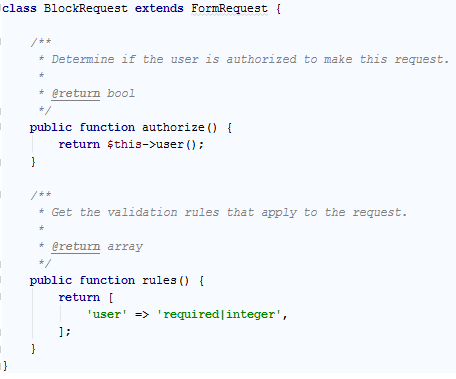
\includegraphics[height=2in]{Images/Testing/BlockRequest}
\caption{Custom request for blocking users}
\label{fig:BlockRequest}
\end{figure}

Figure \ref{fig:BlockRequest} shows an example of one of the custom requests used for blocking a user. In this we can see two functions: one for checking the authorisation of the user making the request and another which includes a set of validation rules. 

\subsection{Permission Testing}
Fidelis is split into accessible pages for authorised and unauthorised users. As such, permissions for page access and actions permissible for a user needed to be tested. This form of testing is important as it deals with the protection of users and their data. The first portion of this testing involved looking at pages that should only be accessible to authorised users. Functionality for checking user authorisation was done by the authentication middleware, but this was tested to make sure it was applied correctly. The remainder of permission testing dealt with verifying requests on a per user basis. This involved checking that a user was permitted to perform the operation they were attempting. For example, user $B$ should not be able to edit or delete posts made by user $A$. Additionally, only user $A$ should be able to modify their settings.

\section{User Acceptance Testing}
User Acceptance Testing (UAT) is one of the last stages of the software development lifecycle, and is performed on the end-user of a given product to gain feedback and approcal on the final product \cite{EconomicTimes:UAT}. UAT is an important part of overall testing and from it, it is possible to identify bugs and gain useful insights into the system and how users view it. This section will look at how UAT was conducted for this project, and in particular will focus on the feedback received from users.

\subsection{User Feedback}
The entire system relies on a stable and growing user base; without the users the system would be rendered useless. With this in mind, guaranteeing a more than satisfactory user experience was an integral system success, and it was therefore important to gain user feedback on the user experience offered by Fidelis. By correctly analysing feedback received from users, system strengths and weaknesses could be used to identified for each progressive system prototype. A number of users were consulted after being given access to the system at various stages of development in order to identify any issues that users may have with the system so that these could be dealt with in latter development stages.

At various stages of the system users were given questionnaires along with a list of tasks to complete. Once the users completed each task, they would answer the questions corresponding to the tasks. No guidance was given to the user and they were expected to use their intuition to navigate the system and perform the tasks. The survey not only included questions on system navigation, but also had questions related to UI design, recommendations and settings provided for privacy and security. Figure \ref{fig:UATQuestionnaire} shows part of the survey given to users after development was completed. The survey accepted a combination of multiple choice and written answers. Multiple choice questions were used to gauge overall user consensus, whereas as written answers provided more detailed feedback on specific system components.

\begin{figure}[H]
\centering
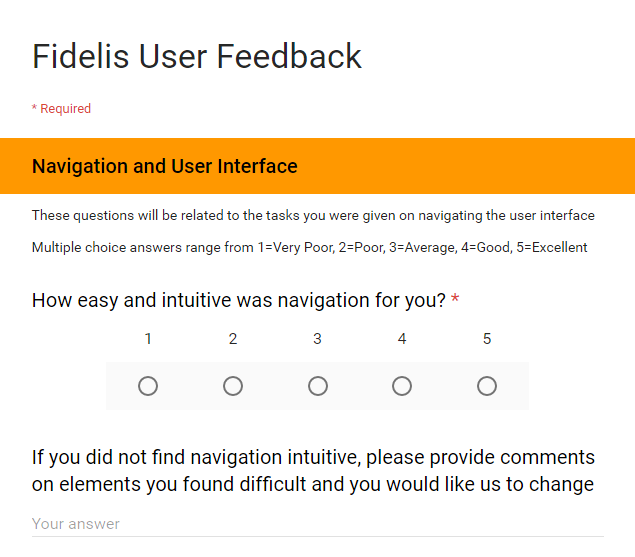
\includegraphics[height=3in]{Images/Testing/UATQuestionnaire}
\caption{Section from final questionnaire given to users as part of UAT}
\label{fig:UATQuestionnaire}
\end{figure}

As mentioned previously, Fidelis design adopted a lot of design elements from Twitter. As a result of this, users felt very comfortable navigating through and using Fidelis. Feedback received, mostly orally, highlighted that the system did need to re-design elements of the UI as it felt and looked too similar to Twitter. A discussion of UI re-design is included in Chapter \ref{Chapter:Conclusion}. Users were very receptive towards the idea of controlling how recommendations were generated for them. By being able to specify a method for recommendations, users were enabled to buy into the idea of Fidelis being a platform that enables them to engage with content they are interested in and have control over. Similar sentiments were voiced on the ability to fine-tune how abuse detection and reputation scoring was conducted.

Acceptance testing played a key role in the development process of the system. Prototypes were built and presented to the user which they evaluated and the feedback from the users was then incorporated into the next iteration of the users. Often a different selection was used to provide an unbiased feedback as existing users would be familiar with the system after previous tests. However, on the final acceptance testing of the complete system, a mix of new and existing users were requested to test the system to see what new users thought about the final product as well as how existing users thought the system had improved.

\subsection{Testimonials}
In this section we look at some of the testimonials received from users. Testimonials were important to collect as they not only give attestation to the success of the system, but also offer up constructive criticisms that will be useful for further system development.

\begin{displayquote}
	\enquote{\textit{It's really interesting how Fidelis is aiming to tackle the issues which exist in social networking. It is definitely a site I would be interested in using, although it will be difficult for it to replace the big names such as Facebook and Instagram in terms of marketing.}}
	
	- Mark Hurdley, University of Warwick MMORSE
\end{displayquote}

\begin{displayquote}
	\enquote{\textit{Fidelis is the whole package. A clever idea, backed up with a clean and intuitive design. Aside from the stark similarity to Twitter this idea can definitely go places.''}}
	
	- Joshua Greenwood, University of Cambridge MPhil
\end{displayquote}

\begin{displayquote}
	\enquote{\textit{Fantastic project.}}
	
	- Luke Vincent, Technology Analyst Barclays PLC
\end{displayquote}

\section{System Tuning and Assessment}